\documentclass[a4paper]{article}

\usepackage[english]{babel}
\usepackage[utf8]{inputenc}
\usepackage{amsmath}
\usepackage{graphicx}
\usepackage[colorinlistoftodos]{todonotes}
\usepackage[numbers]{natbib}

\title{How consistent are macroevolutionary and community ecology patterns of interspecific competition?}

\author{Marina C. Rillo} %, Mauro T. C. Sugawara, Rafael Lopes, \\ Michal Kucera, Thomas H. G. Ezard \& Brenno Cabella}

\date{\today}

\begin{document}
\maketitle

\begin{abstract}


\end{abstract}

%----------------------------------------------------------------------------------------
%%%%%%%%%%%%  INTRODUCTION  %%%%%%%%%%%% 
\section{Introduction}
\label{sec:introduction}

% Ver commentarios Toshiba!


% Criticas Schluter e Pennell: ideias antiquadas,decada 80, devia testar com experimentos - JUSTIFICAR pq nao fiz isso:

% na intro: 
% (1) seria importante primeiro saber o que rola no mano-a-mano, pq no fundo nao sabemos o quanto de niche overlap essas especies tem, e no mano-a-mano seria um jeito de testar. O jeito ideal seria testar com experimentos de microcosmo, que a galera inclusive faz para protists,mas que com forams nao rola pq eles nao sao “cultivaveis” e isso tambem implica no nosso pequeno conhecimento da life history e ecology de plank forams
% (2) por isso testamos throughout a species range, que tambem eh importante pq a gente espera que sera nessa escala que uma especie afetaria a diversificacao da outra

% e ai na discussao posso falar de experimentos (chemiostatos) nos oceanos, em vez de no lab, que esse talvez seja o next step


%%% Macroevolution and community ecology - different scales

The interplay of ecological and evolutionary processes is central to our understanding of biodiversity patterns.
This connection is well accepted, but we still lack a powerful theory for how population-level processes scales up to clade-level dynamics, and vice versa \citep{jablonski2008biotic, weber2017evolution}.
One of the main reason this integration is still missing, is because community ecology and macroevolutionary patterns differ in temporal, spatial and taxonomic scales (Jablonski 2008, Weber 2017 and more refs). 
Community ecology, on the one hand, focusses on local and regional processes, happening along the life-span of individual organisms (which could range from hours to decades). The community is defined taxonomically as the species that co-occur in space and time, and therefore includes species from distantly related clades, from unicellular bacteria and protists to multicellular funghi, animal and plants. 
Macroevolution, on the other hand, focusses on processes that affect the diversification of species. The time scale is millions of years, scaled to the "life-span" of species, and the spatial scale encompasses species' ranges, which can be global. Moreover, macroevolution studies usually focus on monophyletic clades, and therefore species that share more recent evolutionary (and are taxonomically closer) when compared to species that live together in a community. 



%%% Eco-evolutionary feedbacks - the link between ecology and evolution

Although community ecology and macroevolution describe and seek to understand patterns at different scales, the processes generating these patterns are fundamentally linked through eco-evolutionary feedbacks. % focus on both biotic and abiotic factors!
Ecological interactions, which happen at the community scale, are known to shape species’ population dynamics (ref), alter natural selection (ref), and impact trait evolution (ref) and lineage diversification (DDD refs and others). % eco --> evo
Species evolution and diversification, in turn, respond to the changing environment and affect how species interact with the environment and with each other (refs, and more examples). % evo --> eco 
Even knowing that both abiotic and biotic factors play key role in community dynamics and clade diversification, the different scales of the observed patterns makes it hard to test hypothesis relevant to both fields.
% Attempts to integrates these two fields includes...
A promising avenue of research, however, includes contrasting predictions from accepted theories within macroevolution and ecology \citep{voje2015role}.
% A way forward to a mechanistic integration of these fields, however, is to contrast predictions from accepted theories within ecology and macroevolution \citep{voje2015role}.



%%% Diversity-dependent diversification theory --> mechanism: competition among species
% hard to directly test for biotic interactions in the fosil record
Within macroevolution theory, there is the hypothesis that higher levels of diversity tend to suppress rates of diversification (negative diversity-dependence diversification, DDD) (Sepkoski 1978; for a recent debate read: \citealt{harmon2015unbounded} and \citealt{rabosky2015limits}). 
DDD is used to describe both a pattern and a process within macroevolution \citep{rabosky2013diversity}. 
As a pattern, DDD describes a clade's bounded diversity trajectory through time (observed in the fossil record: Sepkoski 1978; Ezard 2011, 2016; and inferred from molecular filogenies: refs) and/or a negative relationship between standing taxonomic richness and rates of diversification across a clade's history (Foote 2018, Alroy, Quental).
As a process, DDD is usually thought to reflect competition among ecologically similar species and the filling of niche space (refs, but see Moen and Morlon TREE). This mechanism also explains species richness rebounds after mass extinctions events (refs), and has been tested by comparing predictions of the DDD and alternative diversification models, including models in which diversification is a function of temperature and rock sedimentation (Ezard 2016, Silvestro PNAS?, achar mais - ver filogenias molecular)(include Marshall and Quental 2016 somewhere).
Although the DDD patterns and models evoke competition among species, they do not explicitly test it, neither reveal how biotic interactions generated them \citep{jablonski2008biotic}. 
Explicitly testing for biotic interactions in the fossil record requires not only a high resolution fossil record (to get closer to temporal scales of community dynamics), but also an actual fossilized interaction proxy, both of which are so rare that until today only one study exists (Liow 2016 PRSB).
% What about works testing for niche saturation using trait evolution? 
% What about network studies, coevolution?


%%% Competition among species happens at the community level
% population-level traits that affect diversificaiton: abundance, range, connectivity...
To generate more mechanistic models of DDD, we need a better understanding of how and under what geographical and environmental circumstances species affect each others' diversification rates (i.e., speciation minus extinction rates) \citep{weber2017evolution}.  
Competitive interactions happen at the individual level. By competing with each other, individuals shape the dynamics of their populations and communities. Population dynamics, in turn, is directly linked to species' abundance and geographical range. And both, species' abundance and geographical range, influences species' diversification rates (Harnik 2011 PNAS, more refs). 
% Competition among species (i.e., interspecific) happens at the community level and is though to affect diversification of whole clades (DDD). 
At the community ecology scale, clade-wide interspecific competition is also hard to test, because you would need geographical and temporal data on population abundances of all (or most) species within a clade. 
Since it is hard to explicitly test for ecological interactions in the fossil record and observe clade-wide community dynamics, the empirical basis for an integration between community ecology and macroevolution theories has thus far been limited (e.g. molluscs; Jablonski et al., 2003, 2013).



%%% Microfossils as a model
Planktonic foraminifera (PF) represent a useful model system for such an integrative research (Yasuhara 2015 Bio Rev). PF are rhizarian protist that build a calcite shell, featuring the most complete fossil record of the Cenozoic Era currently known \citep{kucera2007chapter, ezard2011interplay}. Besides their simple morphology grants them a mature taxonomy, and the extant species are confirm by molecular studies (refs), although some morphospecies might encompass more than one genetic distinct type (cryptic species, refs). 
PF excellent fossil record has been used to test the DDD model. PF speciation rates along the Cenozoic depend on the number of species present at the time, suggesting interspecific competition affects speciation \cite{ezard2011interplay}. % 
More recently, \cite{ezard2016ecolet} showed that the diversification of the PF Cenozoic clade is regulated by competition among species, the strength of which varies through time as a function of environmental change. They invoke niche saturation and competition among species as the underlying mechanisms driving the DDD pattern ,but without explicitly testing for it in the fossil record.
Indeed it is yet not possible to test for PF ecological interactions in the fossil record, because of our lack of understanding of their population dynamics and ecology.
However, PF species live today as zooplankton in the marine pelagic environment, and their low diversity (46 extant morphospecies) allows a clade-wide study of their community dynamics.  
We can expect that, if competition is an important process of PF evolution, competition would also be an important ecological interaction among living PF species. 

%%%
%%% How to test for interspecific competition in today's communities? Communities = snapshot in time
%%%
% For individuals to compete for resources, there should be some level of niche overlap among individuals of the different taxa. 
%% Patterns that would support interspecific competition:
% Allopatry - competitive exclusion takes time, and ghost of past competition
% Correlation time-series

To test for interspecific competition in modern PF asseblages (obs: check use of population, community and assemblage), we analysed PF assemblage data spatially using 4177 assemblage counts around the world's oceans and temporally using 35 time-series collected globally from sediment traps. 
The essence of interspecific competition is that individuals of one species suffer a reduction in fecundity, growth or survivorship as a result of resource exploitation or interference by individuals of another species \citep{begon2006ecology}. This way, competition among individuals affects the population dynamics of the competing species, and these dynamics then influence the species' distributions and diversification. 
Two patters could emerge as ecological effects of interspecific competition: \textit{(i)} species may be eliminated from a habitat by competition from individuals of other species, resulting in a pattern of non-overlapping species’ ranges (i.e. allopatry); or, if competing species coexist, \textit{(ii)} individuals of at least one of them suffer reductions in abundance due to the presence of the other, leading to a pattern of negative correlation of abundances through time.
Sister species are morphogically similar (Supp Info - phylogenetic signal of shell size), thus we assume sister species pairs are ecologically more similar, and therefore compete more strongly, than randomly chosen species pairs. 


%%% Correlation is different than causality
EDM paragraph (correlation of time-series does not imply causality).


%%% Here

% taxonomically and geographically broad database
Here we analyse clade-wide population dynamics of living planktonic foraminifera species using spatial and temporal data to determine how populations of different species interact across their ranges and through ecological time. Given the PF diversity-dependent dynamics in their fossil record \citep{ezard2011interplay, ezard2016ecolet}, we expect interspecific competition to play a key role in structuring modern PF communities. 
% We investigate modern planktonic foraminifera communities and population dynamics to find patterns that would support interspecific competition. 




%%% Readings:

% Weber and Strauss 2016 AREES:On the one hand, the biological similarity and geographic origins of closely related species can promote their co-occurring in the same habitats. On the other hand, close relatives can ecologically, genetically, and reproductively interfere with one another owing to their morphological and ecological similarities. Community ecology generally excludes the deeper phylogenetic history of species pools, ignoring historical biogeography (see critiques by Cornell & Harrison (2014), Mittelbach et al. (2007), Ricklefs (2007)).
% Ecological processes that actually allow populations of species to have stable or positive population growth in sympatry. 
% Here, we define close relatives loosely as relatively recently diverged, morphologically, and/or ecologically similar species. 
% Coexistence requires nuanced consideration of spatial and temporal scale, migration/phenology, and microallopatry (Siepielski & McPeek 2010).
% Speciation and extinction can have prominent roles in shaping patterns of coexistence in close relatives.


% While there is empirical evidence in the fossil and neontological records of diversity dependence at play, we should note that diversity-dependence rates, although necessary, are not sufficient evidence to demonstrate the existence of a fixed carrying capacity [14,18,30,31]. In fact the results shown by Morlon et al. [32] based on several molecular phylogenies suggest that although rates of diversification consistently decrease over time, diversity for those same phylogenies are probably still expanding.

% The traditional diversity-dependent patterns are a negative relationship between standing taxonomic richness and diversification rate or speciation rate, or a positive relationship between richness and extinction rate (Alroy 1996; Wiens 2011; Cornell 2013). These traditional diversity-dependent signatures evoke macroevolutionary competition, but do not reveal how biotic interactions generated them (Jablonski 2008) nor whether a finite upper bound constrains species richness (Marshall & Quental 2016).

% Why just within a clade? Germain 2016, but silvestro quental 2016 PNAS
% Rachel M. Germain 2016: The diversity of ecological interactions on the Earth is the product of approximately 3.5 billion years of evolution, with ongoing extinctions matched by the continual divergence of populations and species. Signatures of this past evolution frequently emerge in the strength of the interactions among current-day species [1] in ways that have potential to further perpetuate divergence and the evolution of interaction strengths [2]. This dynamic feedback between the ecology and evolutionof organisms is a central theme in microevolutionary [3,4], macroevolutionary [5] and recent ecological perspectives [6–8], as it promises a more complete picture of the processes that generate and maintain biological diversity.

% A taxonomic group may limit species diversification or another group and therefore affect its species richness (Silvestro et al 2015), but the underlying mechanism of competition is still the same: individuals compete for resources. Thus the competitive process limiting diversification of whole clades also acts by affecting individual fitness, average population fitness and population size (contrary to line 53). You can think of different levels that competition affects: between individuals and suppresses access to resources, between populations and suppresses population sizes and between higher order taxa and suppresses species richness. However the underlying mechanism is always acting at the individual level. A population size can only be suppressed if their individuals have less access to resources and smaller reproductive success. And a species reduced diversification rate can only be suppressed via its populational sizes and average fitness. The results of these three levels of competition surely occur at different temporal, spatial and taxonomic scales. It takes longer for a species to go extinct than an individual to die. Species ranges are generally larger than individuals’ home ranges. The outcomes are expected to occur in different scales, however the underlying processes are all the same, at the same scale: competition among individuals.





%----------------------------------------------------------------------------------------
%%%%%%%%%%%%  METHODS  %%%%%%%%%%%% 
\section{Methods}


\subsection{Sediments trap data}

Sediments traps consist of an upward-facing funnel that directs sinking organic and inorganic particulate material towards a sampling bottle. 
Traps are moored at a specific depth in the water column (usually below the euphotic zone or mixed layer) and anchored to a particular location. %REF
Each trap usually contains several collecting bottles to record the changes in sinking flux with time, typically at the resolution of weeks. %REF
Therefore, sediment traps provide continuous time series of settling foraminiferal shell fluxes (expressed as number of shells per $m^2$ per day). 

Shell fluxes represent the settling of dead foraminifera and are strictly speaking not directly a measure of abundance of foraminifera in the water column \cite{jonkers2015global}. However, given the short life span of foraminifera (typically one month \citep{hemleben1989modern}), the fluxes are likely to be a good proxy for populational abundance. Moreover, to be able to compare fluxes of different species, we assume that species have similar life spans. This means that similar fluxes (i.e. species dying synchronously) indicate that species grow and reach different life stages (juvenile, adults) also synchronously.

%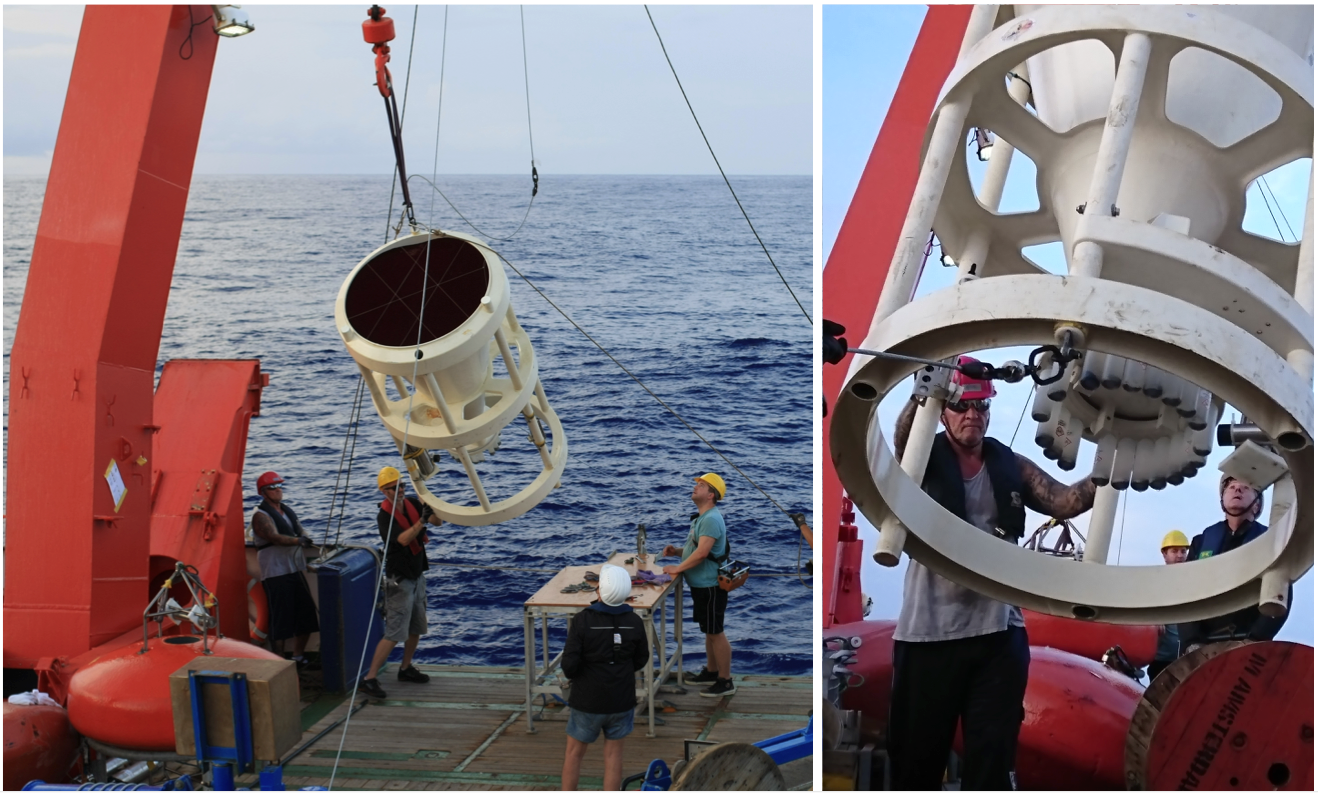
\includegraphics[width=1\textwidth]{sed_trap.png}
%\caption{\label{fig:trap} Recovery of sediment trap during the German Research Cruise M140 in the North Atlantic, crew in the \textit{RV} Meteor, August 2017. \textbf{Left}: sediment trap has a sampling area of $1 m^2$, \textbf{Right}: 20 bottles with samples, note the four missing bottles.}

We used the data of 35 globally distributed moored sediment trap time series (Fig. \ref{fig:map}, compiled by \citealt{jonkers2015global}). All the traps have duration of at least one year; and traps 36 and 37 were excluded from this study because they contain only one polar species. Further information about each trap (\textit{e.g.} location, resolution, total period of sampling) can be found in Table \ref{table:traps_data}. Figure \ref{fig:NB67_series} shows an example of the data gathered by trap no.1 in the North Atlantic. 
% Jonkers 2015: Traps close to the sea floor or in the vicinity of (steep) topography that showed the influence of resuspended material (for instance, the presence of benthic Foraminifera) were not considered. In cases were multiple sediment traps were deployed at different depths on the same mooring, we report data from the shallowest trap as this (likely) reduces the catchment area of the trap and the data hence reflect local conditions more closely.

\begin{figure}
\center
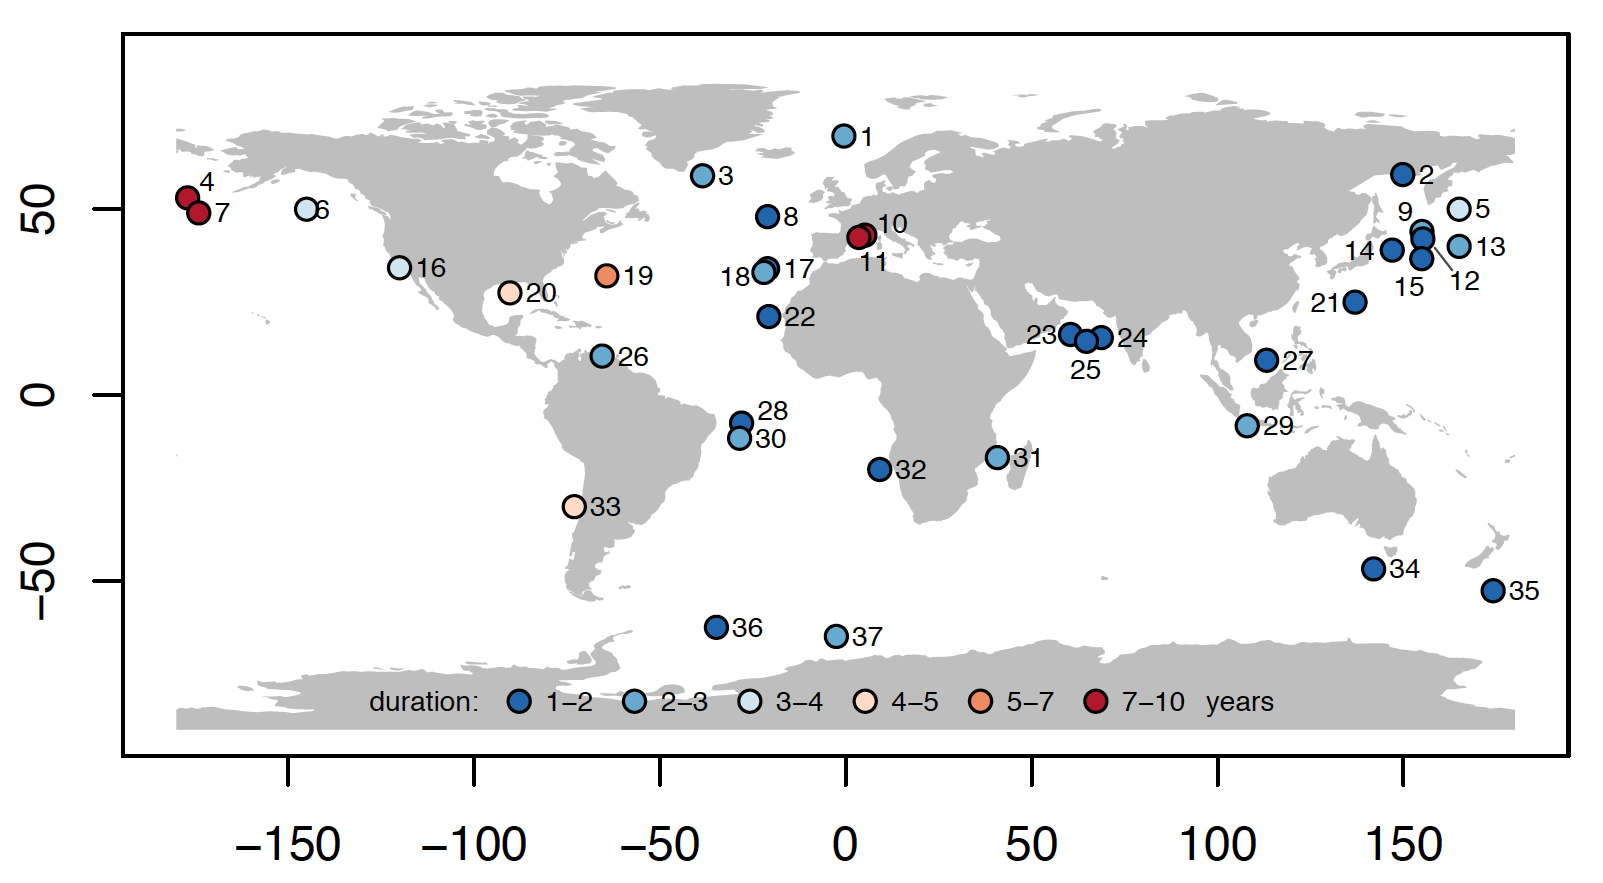
\includegraphics[width=1\textwidth]{chap_competition/traps_map.png}
\caption{\label{fig:map} Distribution and total duration of sediment trap time series used in this study. Figure taken from \citep{jonkers2015global}. Traps 36 and 37 were excluded from this study because they contain only one species. \textcolor{red}{(plot this map myself)}}
\end{figure}

\begin{table}
\center
\footnotesize
\caption{\label{table:traps_data} Meta-data of sediment traps taken from \citep{jonkers2015global}. Columns: \textbf{Trap number} as in Figure \ref{fig:map}; \textbf{Trap name}; Coordinates (\textbf{Lat, Lon}); \textbf{resolution}: mean period (in days) that each sample (bottle) in the trap was open; \textbf{length days}: total period trap was open (in days); \textbf{length years}: total period in years; \textbf{length series}: total number of samples collected in each trap (length of the time-series); \textbf{from, to}: year interval when trap was active; \textbf{all ssp}: whether all species were identified in each trap, "NO" means that just dominant species were picked.}
\begin{tabular}{rlllrrrrrrl}
  \hline
Trap & Trap & Lat & Lon & resolution & length & length & length & from & to & all ssp \\ 
no.  & name &  &  & days & days & years & series &  &   &  \\ 
  \hline
  1 & NB67 & 69.69 & -0.47 & 18.20 & 787 & 2.20 &  32 & 1991 & 1993 & YES \\ 
    2 & OKH & 59.32 & 149.83 & 16.40 & 365 & 1.00 &  21 & 1990 & 1991 & YES \\ 
    3 & IRM & 59.00 & -38.50 & 16.00 & 1372 & 3.80 &  58 & 2003 & 2007 & NO \\ 
    4 & AB & 53.05 & -177.00 & 26.90 & 3264 & 8.90 & 105 & 1990 & 1999 & NO \\ 
    5 & PAC50 & 50.00 & 165.00 & 15.50 & 1287 & 3.50 &  69 & 1997 & 2001 & NO \\ 
    6 & PAPA & 50.00 & -145.00 & 12.80 & 1437 & 3.90 &  82 & 1982 & 1986 & NO \\ 
    7 & SA & 49.00 & -174.00 & 26.80 & 3267 & 9.00 & 101 & 1990 & 1999 & NO \\ 
    8 & JGOFS48 & 48.00 & -21.00 & 12.80 & 377 & 1.00 &  26 & 1989 & 1990 & YES \\ 
    9 & PACKNOT & 44.00 & 155.00 & 15.40 & 893 & 2.40 &  52 & 1997 & 2000 & NO \\ 
   10 & LIP & 43.02 & 5.18 & 27.80 & 4457 & 12.20 & 116 & 1993 & 2006 & YES \\ 
   11 & LIL & 42.41 & 3.54 & 22.50 & 4167 & 11.40 & 151 & 1993 & 2005 & YES \\ 
   12 & WCT6 & 42.01 & 155.24 & 19.10 & 381 & 1.00 &  19 & 1999 & 2000 & YES \\ 
   13 & PAC40 & 40.00 & 165.00 & 16.50 & 952 & 2.60 &  44 & 1997 & 2000 & NO \\ 
   14 & WCT2 & 39.00 & 147.00 & 14.20 & 628 & 1.70 &  40 & 1997 & 1999 & PROB \\ 
   15 & WCT7 & 36.69 & 154.94 & 18.80 & 375 & 1.00 &  19 & 1999 & 2000 & PROB \\ 
   16 & SBB & 34.25 & -120.00 & 10.90 & 2144 & 5.90 &  93 & 1993 & 1999 & NO \\ 
   17 & JGOFS34 & 34.00 & -21.00 & 12.80 & 377 & 1.00 &  26 & 1989 & 1990 & YES \\ 
   18 & L1 & 33.00 & -22.00 & 21.80 & 767 & 2.10 &  35 & 2002 & 2004 & YES \\ 
   19 & BATS & 32.08 & -64.25 & 58.60 & 2232 & 6.10 &  31 & 1978 & 1984 & PROB \\ 
   20 & GOM & 27.50 & -90.30 & 7.30 & 2245 & 6.20 & 238 & 2008 & 2014 & NO \\ 
   21 & WCT1 & 25.00 & 137.00 & 14.10 & 612 & 1.70 &  37 & 1997 & 1999 & PROB \\ 
   22 & CB & 21.13 & -20.67 & 17.90 & 753 & 2.10 &  38 & 1989 & 1991 & NO \\ 
   23 & WAST & 16.32 & 60.47 & 13.30 & 529 & 1.40 &  38 & 1986 & 1987 & YES \\ 
   24 & EAST & 15.47 & 68.75 & 11.70 & 527 & 1.40 &  38 & 1986 & 1987 & YES \\ 
   25 & CAST & 14.47 & 64.75 & 12.20 & 516 & 1.40 &  32 & 1986 & 1987 & YES \\ 
   26 & CAR & 10.50 & -65.50 & 12.40 & 1089 & 3.00 &  75 & 1997 & 1999 & NO \\ 
   27 & SCS & 9.38 & 113.23 & 29.10 & 663 & 1.80 &  22 & 2004 & 2006 & NO \\ 
   28 & WA3 & -7.52 & -28.00 & 24.00 & 499 & 1.40 &  20 & 1993 & 1994 & NO \\ 
   29 & JAM & -8.25 & 108.00 & 16.20 & 983 & 2.70 &  56 & 2000 & 2003 & PROB \\ 
   30 & WAB & -11.60 & -28.53 & 23.80 & 1001 & 2.70 &  38 & 1997 & 1999 & NO \\ 
   31 & MOZ & -16.80 & 40.80 & 20.90 & 862 & 2.40 &  39 & 2003 & 2006 & NO \\ 
   32 & WR23 & -20.00 & 9.16 & 17.70 & 751 & 2.10 &  28 & 1989 & 1991 & NO \\ 
   33 & COQ & -30.00 & -73.00 & 8.80 & 2679 & 7.30 & 159 & 1994 & 2001 & NO \\ 
   34 & SAZ47 & -46.75 & 142.00 & 10.60 & 493 & 1.40 &  40 & 1997 & 1999 & PROB \\ 
   35 & CP & -52.62 & 174.15 & 8.80 & 425 & 1.20 &  42 & 1998 & 1999 & NO \\ 
   %36 & WS1 & -62.45 & -34.76 &  &  &  &  &  &  & NO \\ 
   %37 & WS34 & -64.90 & -2.50 &  &  &  &  &  &  & NO \\ 
   \hline
\end{tabular}
\end{table}


%----------------------------------------------------------------------------------------
\subsection{Co-occurrence of species}

To test whether species overlap in their ranges, I simply recorded whether two species were sampled at the same time in the same sediment trap, or whether they were never found together in the same collecting bottle. If species were sampled together at least once, they co-occur (live in sympatry). 

%----------------------------------------------------------------------------------------
\subsection{Correlation of time-series}

For the species that did co-occur, we tested whether their changes in abundances are positively or negatively correlated through time. To record the change in species abundances from one time step to the next, we calculated the first differences of each time-series. Additionally, this method reduces the time-series autocorrelation. %  time series of the first-differenced values
%This give us a series of the change in abundance from one time-step (sample) to the next. 
First differences were not calculated for consecutive samples between which there was a sampling gap of more than 10 days. The reason is that if the sediment trap did not sample for a specific period (\textit{e.g.} a collecting bottle was lost), there was no recording of the abundance flux for that period, and thus the first difference of the two adjacent samples does not record the change in abundance from one time-step to the next.

Next, for each trap, we calculated for each species pair the non-parametric Kendall correlation of the differentiated series (for example, Fig. \ref{fig:NB67_series} for trap no.1). This correlation does not rely on any assumptions on the distributions of the time-series (Note: Pearson and Spearman correlations show similar overall results). 

Finally, we wanted to see the overall species abundances patterns for all 35 sediment traps, noting that species can behave differently in different environments (sediment traps). For each species pair, we calculated the proportion of significant positive and negative correlations considering the total number of sediment traps they both co-occurred.


%----------------------------------------------------------------------------------------
\subsection{Null model (surrogates)}
The positive correlation among species might be an effect of seasonality. 
% another way to solve: function decompose in R,decompor a série temporal como uma soma de (trend + seasonality + noise) e subtrair a componente sazonal antes de fazer a análise. Porem, to do this, precisa botar a série no formato "time-series" do R. pra isso eh so usar a função "ts()", mas vc vai precisar saber o periodo (freq) da série.Pra achar o período, se não for nada óbvio (tipo anual) dá pra tentar chutar olhando as funções de autocorrelação e autocorrelação parcial (adf() e pacf() no R)
% "partial correlation": "the correlation between the residuals RX (X=ssp1) and RY (Y=ssp2) resulting from the linear regression with Z (Z = temperatura)"

For each time-series (\textit{i.e.}, each species in each sediment trap) we calculated a smoothing spline of the shell fluxes based on yearly observations. To do this, the observations were put on the same time-scale by converting the first date of the collection intervals to the day of the year. Then, a spline function was applied to the data.
We do not need to impose a priori the seasonality of the data with this methodology,and it allows for any number of shell flux peaks throughout the year.

The correlation between the time-series raw data and the spline series is an indicator of how seasonal the variable is. SST, for example, shows always a high correlation ($\rho$ ~ 0.9). We assume that if a species' shell flux responds to SST(or any other variable that relates to SST), its time-series will also be seasonal and show a high correlation with its splines. 

We generated a null model based on the splines of each time-series. For each time-step, we calculated the residual between the time-series data and the spline data, resulting in a vector of residuals with the same length as the time-series and the spline series. We then randomized the residuals 500 times (\textit{i.e.}, 500 different vectors) and added it to the base spline series. This resulted in 500 null series. We calculated the correlation between species pairs for this 500 null series, and the resulting correlation distribution was used as the null model which takes seasonality into account. 

If species correlate positively just because they have synchronous seasonality, then their splines should correlate positively as well. 



%----------------------------------------------------------------------------------------
%%%%%%%%%%%%  Results  %%%%%%%%%%%% 
\section{Results}

\subsection{Co-occurrence of species}

The majority of species co-occur (Fig. \ref{fig:co-occur}). The species that often do not co-occur with other species are rare species (\textit{i.e.} present in less than 5\% of the samples). PF float passively in the highly-connected pelagic environment, thus we expected most PF species to co-occur.

\begin{itemize}
\item How many times and where do species co-occur? Build a co-occurrence matrix based on frequency of co-occurrences (instead of just single-tons 0 and 1 as in Fig \ref{fig:co-occur}).
\item Strength of the co-occurrence $~$ resolution sediment trap (2 months open, everybody co-occurs)
\item Take depth habitat into account. Species may fall in the same sediment trap (sympatry here) but actually live in different depths of the water column (and thus in allopatry).
\item Take cryptic (genetic) species biogeography into account. Some genetic types show allopatric geographical patterns. Maybe competition acts at this level?
\end{itemize}

\subsubsection{Problems}
Null model: it is hard to build a null model of plankton spatial distribution, especially taking abundance into account (instead of just presence/absence). Many of the environmental variables covary and ocean currents have to be taken into account.



\subsection{Correlation of time-series}

The majority of the correlations between species pairs were positive (Fig. \ref{fig:corr_prop})

\begin{itemize}
\item Strength of the correlation $~$ resolution sediment trap (2 months open, everybody co-occurs)
\item Calculate correlations of one species against all other species in the community (instead of just pairs of species)
\item How do the patterns change when doing this for relative abundances (as in the fossil record)? 
\item Are the species with higher abundances in the time-series always the same? (are they always the "winners"?)
\end{itemize}


\subsubsection{Problems} 
How to test if this overall positive correlation is not expected due to, for example, phytoplankton seasonality? How to build a null model of abundances time-series? My idea would be to somehow take out the variance explained by environmental data (temperature and primary productivity) and then try to correlate the residuals.

\begin{figure}
\centering
\includegraphics[width=0.7\textwidth]{chap_competition/traps_co-occur.png}
\caption{\label{fig:co-occur} Co-occurrence matrix. In blue: species that co-occurred at least in one samples. The species names are positioned to indicate the columns and rows that represent their pairwise co-occurrence with other species. The matrix is clustered accordingly to the incidence of species on the samples; rarely sampled species are shown in red and were found in less than 5\% of the total samples.}
\end{figure}

\begin{figure}
\centering
\includegraphics[width=0.8\textwidth]{chap_competition/traps_correlation_low.png}
\caption{\label{fig:corr_prop} Proportion of significant positive (upper triangle, blue) and negative (lower triangle, red) correlations between first differences of time-series in which both species occur. White squares represent species pairs that co-occur but showed no significant positive and/or negative correlation. The black crosses indicate species pairs that did not co-occur.}
\end{figure}

%----------------------------------------------------------------------------------------
%----------------------------------------------------------------------------------------
%%% DISCUSSION
\section{Discussion}


% We found a positive correlation among species abundances through time and space, contrary to the community assembly patterns expected under strong interspecific competition. 
We found no evidence for interspecific competition structuring planktonic foraminifera communities. Thus there seems to be a mismatch between the processes inferred from macroevolutionary patterns over deep time and those inferred from ecological patterns observed in a shorter time scale. This means that either macroevolutionary processes are different than the current the ecological processes, or that interspecific competition might not be the mechanism underlying the patterns seen in the fossil record.

Scale problem: competition takes time, competition at ecological scales might generate diversification at evolutionary scales. 
Intraspecific competition promotes diversification theoretically (Doebeli, adaptive dynamics) and experimentally (Bailet et al. 2013 bacteria, increased richness, increased diversification; check david's intro as well) - what about interspecific competition? Niche partitioning / specialization first step to species diversification
Jablonski 2008: competition at the community scale might not have negative impact at the macroevolutionary scale.


A promising avenue of research, however, includes contrasting predictions from relevant theories within ecology and macroevolution, as well as embracing both abiotic and biotic proxies while modelling long-term evolutionary data \citep{voje2015role}. Biotic and abiotic affects population dynamics.

An important shortcoming of microfossils, for example compared to molluscs, is insufficient knowledge of their basic biology and natural history. Yet this current weakness is balanced by some distinctive strengths of the microfossils record, such as high abundance, large spatio-temporal coverage, and good taxonomic and temporal resolution (Yasuhara 2015).

Planktonic foraminifera (PF) unique fossil record has been used to test the diversity-dependent diversification model. PF speciation rates along the Cenozoic depend on the number of species present at the time, and decline as the number of species increases (DDD pattern), whereas extinction rate was driven largely by climate \cite{ezard2011interplay}. % 
More recently, \cite{ezard2016ecolet} showed that the diversification of the PF Cenozoic clade is regulated by competition among species, the strength of which varies through time as a function of environmental change. They invoke niche saturation and within-clade interspecific competition as the underlying mechanisms driving the DDD pattern without explicitly testing for it in the fossil record (because it is not possible actually).
% ezard2016ecolet:
% PF diversification dynamics is regulated by biotic "compensatory contest" competition, meaning that a constant number of successful individuals get the precise amount of resource they require, which is a fixed quantity (instead of the limiting resource being shared equally among all competing individuals - "scramble competition").
% temperature affects the per-lineage diversification rate, while both temperature and an environmental driver of sediment accumulation defines the carrying capacity
% contest competition constrains species richness by restricting niche availability, and that the number of macroevolutionary niches varies as a function of environmental changes.

A group may have more potential for coexistence among close relatives simply because that lineage has been present in that area for a longer amount of time.


%----------------------------------------------------------------------------------------

\section{Methods}
\label{sec:methods}

\subsection{Gulf of Mexico sediment trap}
The Gulf of Mexico (GoM, 27.5N -90.3E (= 269.7), \textcolor{red}{REF}) sediment trap has the best resolution of all the sediment traps compiled by \cite{jonkers2015global}. The resolution is one community sample every 7 days (\textit{i.e.} each sample represents the accumulation of foraminifera shells of the previous week). The total length of the GoM time-series is 238 samples, spanning over 2245 from 14th January 2008 to 8th March 2014.

\subsection{Temperature for the Gulf of Mexico sediment trap}
I used the dataset NOAA 1/4o daily Optimum Interpolation Sea Surface Temperature (or daily OISST, AVHRR-Only) \citep{smith2016oisst}.  % http://monitor.cicsnc.org/obs4MIPs/    https://www.ncdc.noaa.gov/oisst/data-access 
We used the temperature data point of coordinates (lon 269.625  lat 27.625) 15,76 km away from the sediment trap. 

I calculated the mean of the daily temperature for each sampling interval. The NOAA dataset has the temperature values in Kelvin, the Celsius column was created subtracting 273.15 from the Kelvin values. 
% Uma coisa a se pensar é que nossos dados da serie temporal são conchas de foraminiferos que morreram recentemente. Então, o indivíduo que morreu no dia X (ou antes do dia X, e só caiu na armadilha no dia X), não vivenciou a temperatura do dia X e sim dos dias anteriores. Como o tempo de vida médio de um indivíduo é um mês (obs.: isso não é completamente claro na literatura/campo), talvez seja melhor eu colocar os dados de temperatura de X-15 dias ou ate X - 30 dias. Eu poderia ja adicionar uma coluna extra tipo "temp_oC-15days". O que vocês acham?


\subsection{Empirical dynamic modelling and convergent cross mapping}
Empirical dynamic modelling (EDM) and convergent cross mapping (CCM), R package rEDM.



%----------------------------------------------------------------------------------------

\section{Results}
\label{sec:results}

\subsection{Co-occurrence of species}

The majority of species co-occur (Fig. \ref{fig:co-occur}). The species that often do not co-occur with other species are rare species (\textit{i.e.} present in less than 5\% of the samples). PF float passively in the highly-connected pelagic environment, thus we expected most PF species to co-occur.

\begin{itemize}
\item How many times and where do species co-occur? Build a co-occurrence matrix based on frequency of co-occurrences (instead of just single-tons 0 and 1 as in Fig \ref{fig:co-occur}).
\item Strength of the co-occurrence $~$ resolution sediment trap (2 months open, everybody co-occurs)
\item Take depth habitat into account. Species may fall in the same sediment trap (sympatry here) but actually live in different depths of the water column (and thus in allopatry).
\item Take cryptic (genetic) species biogeography into account. Some genetic types show allopatric geographical patterns. Maybe competition acts at this level?
\end{itemize}

\subsubsection{Problems}
Null model: it is hard to build a null model of plankton spatial distribution, especially taking abundance into account (instead of just presence/absence). Many of the environmental variables covary and ocean currents have to be taken into account.



\subsection{Correlation of time-series}

The majority of the correlations between species pairs were positive (Fig. \ref{fig:corr_prop})

\begin{itemize}
\item Strength of the correlation $~$ resolution sediment trap (2 months open, everybody co-occurs)
\item Calculate correlations of one species against all other species in the community (instead of just pairs of species)
\item How do the patterns change when doing this for relative abundances (as in the fossil record)? 
\item Are the species with higher abundances in the time-series always the same? (are they always the "winners"?)
\end{itemize}


\subsubsection{Problems} 
How to test if this overall positive correlation is not expected due to, for example, phytoplankton seasonality? How to build a null model of abundances time-series? My idea would be to somehow take out the variance explained by environmental data (temperature and primary productivity) and then try to correlate the residuals.

\begin{figure}
\centering
\includegraphics[width=0.7\textwidth]{traps_co-occur.png}
\caption{\label{fig:co-occur} Co-occurrence matrix. In blue: species that co-occurred at least in one samples. The species names are positioned to indicate the columns and rows that represent their pairwise co-occurrence with other species. The matrix is clustered accordingly to the incidence of species on the samples; rarely sampled species are shown in red and were found in less than 5\% of the total samples.}
\end{figure}

\begin{figure}
\centering
\includegraphics[width=0.8\textwidth]{traps_correlation_low.png}
\caption{\label{fig:corr_prop} Proportion of significant positive (upper triangle, blue) and negative (lower triangle, red) correlations between first differences of time-series in which both species occur. White squares represent species pairs that co-occur but showed no significant positive and/or negative correlation. The black crosses indicate species pairs that did not co-occur.}
\end{figure}


%----------------------------------------------------------------------------------------
\newpage

\section{Discussion}
\label{sec:discussion}
%%% DISCUSSION

% We found a positive correlation among species abundances through time and space, contrary to the community assembly patterns expected under strong interspecific competition. 
We found no evidence for interspecific competition structuring planktonic foraminifera communities. Thus there seems to be a mismatch between the processes inferred from macroevolutionary patterns over deep time and those inferred from ecological patterns observed in a shorter time scale. This means that either macroevolutionary processes are different than the current the ecological processes, or that interspecific competition might not be the mechanism underlying the patterns seen in the fossil record.

Scale problem: competition takes time, competition at ecological scales might generate diversification at evolutionary scales. 
Intraspecific competition promotes diversification theoretically (Doebeli, adaptive dynamics) and experimentally (Bailet et al. 2013 bacteria, increased richness, increased diversification; check david's intro as well) - what about interspecific competition? Niche partitioning / specialization first step to species diversification
Jablonski 2008: competition at the community scale might not have negative impact at the macroevolutionary scale.


A promising avenue of research, however, includes contrasting predictions from relevant theories within ecology and macroevolution, as well as embracing both abiotic and biotic proxies while modelling long-term evolutionary data \citep{voje2015role}. Biotic and abiotic affects population dynamics.

An important shortcoming of microfossils, for example compared to molluscs, is insufficient knowledge of their basic biology and natural history. Yet this current weakness is balanced by some distinctive strengths of the microfossils record, such as high abundance, large spatio-temporal coverage, and good taxonomic and temporal resolution (Yasuhara 2015).

Planktonic foraminifera (PF) unique fossil record has been used to test the diversity-dependent diversification model. PF speciation rates along the Cenozoic depend on the number of species present at the time, and decline as the number of species increases (DDD pattern), whereas extinction rate was driven largely by climate \cite{ezard2011interplay}. % 
More recently, \cite{ezard2016ecolet} showed that the diversification of the PF Cenozoic clade is regulated by competition among species, the strength of which varies through time as a function of environmental change. They invoke niche saturation and within-clade interspecific competition as the underlying mechanisms driving the DDD pattern without explicitly testing for it in the fossil record (because it is not possible actually).
% ezard2016ecolet:
% PF diversification dynamics is regulated by biotic "compensatory contest" competition, meaning that a constant number of successful individuals get the precise amount of resource they require, which is a fixed quantity (instead of the limiting resource being shared equally among all competing individuals - "scramble competition").
% temperature affects the per-lineage diversification rate, while both temperature and an environmental driver of sediment accumulation defines the carrying capacity
% contest competition constrains species richness by restricting niche availability, and that the number of macroevolutionary niches varies as a function of environmental changes.

A group may have more potential for coexistence among close relatives simply because that lineage has been present in that area for a longer amount of time.


%----------------------------------------------------------------------------------------

\label{Bibliography}
\bibliographystyle{abbrvnat} % Use the agsm, abbrvnat, unsrtnat BibTeX style for formatting the Bibliography
\bibliography{gom-bibliography.bib} % The references (bibliography) information are stored in the file named "Bibliography.bib"

\end{document}  

